\documentclass[10pt,a4paper]{amsart}
\usepackage[margin=19mm]{geometry}
\usepackage{amsmath,amssymb,mathtools}
\usepackage[scr=rsfs,cal=euler]{mathalfa}
\usepackage{xfrac}
\usepackage[unicode,hidelinks,bookmarks=false]{hyperref}
\newcommand{\ie}{i.e.\ }
\newcommand{\cf}{cf.\ }
\newcommand{\resp}{respectively\ }
\newcommand{\Subsection}{\subsection}
\providecommand{\nobreakdash}{\nobreak\hbox{-}}
\setlength{\emergencystretch}{2em}
\multlinegap0pt
\usepackage{mdframed}
\usepackage{mdframed}
\usepackage{mdframed}
\usepackage{mdframed}
\usepackage{tikz}
\usepackage{amssymb}
\usepackage{enumerate}
\usepackage[shortlabels]{enumitem}
\usepackage{algorithm}\usepackage{algpseudocode}
\usepackage{mdframed}
\usepackage{tcolorbox}
\usepackage{xcolor}
\newtheorem{corollary}{Corollary}
\newtheorem{proposition}{Proposition}
\newtheorem{remark}{Remark}
\newtheorem{example}{Example}
\usepackage{cleveref}
\crefname{corollary}{Corollary}{Corollarys}
\crefname{proposition}{Proposition}{Propositions}
\crefname{remark}{Remark}{Remarks}
\crefname{example}{Example}{Examples}
\newcommand{\Z}{\mathbb{Z}}
\title{Invariants of Legendrian knots in thickened convex surfaces}
\author{Nancy Mae Eagles, Zijian Rong}
\date{Source: arXiv:2604.22053v2 (CC BY 4.0)}
\begin{document}
\maketitle

\noindent\emph{Source and licence.} Invariants of Legendrian knots in thickened convex surfaces. Version arXiv:2604.22053v2 (CC BY 4.0), distributed by arXiv under the Creative Commons Attribution 4.0 International licence, http://creativecommons.org/licenses/by/4.0/, as recorded in the arXiv licence metadata for this exact version and shown on the abstract page https://arxiv.org/abs/2604.22053v2. Full licence notice: \texttt{licenses/arxiv-2604.22053-CC-BY-4.0.txt}.\par\smallskip

\noindent\textit{Editorial scope.} Counted unit: the article's proposition prop:phipmDGA (source0.tex lines 3262--3264). The article's complete original proof of it is delivered with it (source0.tex lines 3266--3733, one \texttt{proof} environment of 468 lines). No mathematics is written, repaired or re-derived: the statement and the proof are the article's own lines, in the article's own notation, and no retained line is substituted or re-flowed.  Retained uncounted as the source-local context the proof needs: lines 2492--2494; lines 3735--3892.  Nothing was omitted from any retained span, so the package carries no omission record.  No retained line contains a citation, so the wrapper carries no bibliography and no bibliography entry.  The retained lines contain the article's own diagram code, which the wrapper typesets with the standard tikz packages; no image file is delivered and the package declares no asset dependency.  Editorial formatting only, in addition: an AMS \texttt{amsart} preamble that restates the article's own declarations and macros used by the retained lines, namely the environments \texttt{corollary}, \texttt{proposition}, \texttt{remark}, \texttt{example} on separate counters, together with the standard packages those lines need.  The retained environments print in this document as Corollary 1, Proposition 1, Remark 1, Example 1 in order of appearance, whereas the article prints the same items with the numbering of its own full document.  The complete native source of the article as distributed in the arXiv e-print for this exact version is bundled unchanged as \texttt{sources/199065/source0.tex}.
\begin{corollary}\label{cor:phipmgrading}
    $\Phi_\pm: \mathcal{A}_\Gamma \rightarrow \mathcal{A}_\pm$ preserves the grading.
\end{corollary}

\begin{remark}\label{rem: why hypertight} Suppose that $\text{start}(w) = \text{end}(w)$. Consider a monomial $v\in \Phi_+\circ \partial_\Gamma(w)$. Then the coefficient of $v$ is a count of rigid polygons of the form in \Cref{fig:hypertight 1}. Note in particular that the two disks share two boundary arcs, $\gamma$ and $\gamma'$, which  may coincide. If they do not coincide, then at least one disk must have a negative asymptotic end in $\Sigma_+$. In this case, the argument proceeds identically to that in the proof of \cref{prop:phipmDGA}. If $\gamma$ and $\gamma'$ do coincide, then $\Lambda$ must have the configuration shown in \cref{fig:hypertight 3}. We may think of this case as a degeneration of a disk along an obtuse corner on $\Gamma$ at $\text{start}(w') = \text{end}(w'')$. For such a disk there is only one possible degeneration, which would imply that $\Phi_+$ is not a chain map. We can circumvent this problem by noting that the concatenation of the two disks is a disk whose boundary is $w$, so that $w$ a contractible Reeb orbit. Restricting to the case that $\xi$ is hypertight eliminates this possibility. 

\begin{figure}[h]
    \begin{minipage}{0.48\textwidth}
        \centering
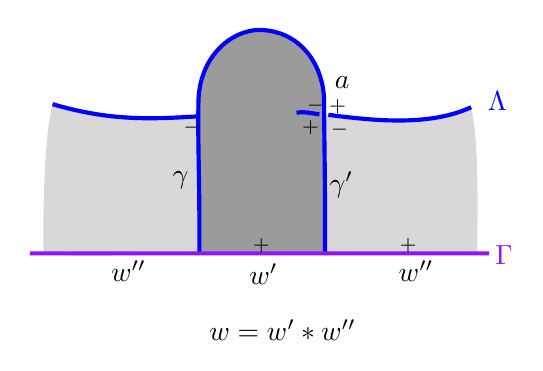
\begin{tikzpicture}[x=0.55pt,y=0.55pt,yscale=-1,xscale=1]
%uncomment if require: \path (0,300); %set diagram left start at 0, and has height of 300

%Shape: Polygon Curved [id:ds18864319797586704] 
\draw  [draw opacity=0][fill={rgb, 255:red, 216; green, 216; blue, 216 }  ,fill opacity=1 ] (437.79,103.57) .. controls (414.04,113.85) and (362.79,112.57) .. (341.97,108.54) .. controls (341.76,139.16) and (343.69,173.61) .. (341.73,198.61) .. controls (364.4,200.71) and (410.85,199.74) .. (441.79,198.57) .. controls (442.17,159.74) and (442.5,124.92) .. (437.79,103.57) -- cycle ;
%Shape: Polygon Curved [id:ds20416456082559908] 
\draw  [draw opacity=0][fill={rgb, 255:red, 216; green, 216; blue, 216 }  ,fill opacity=1 ] (162.79,101.57) .. controls (191.79,111.57) and (240.63,108.77) .. (259.97,109.54) .. controls (257.79,140.67) and (257.79,173.67) .. (259.79,198.67) .. controls (236.63,200.77) and (188.39,201.74) .. (156.79,200.57) .. controls (156.39,161.74) and (157.79,120.57) .. (162.79,101.57) -- cycle ;
%Rounded Same Side Corner Rect [id:dp5510477202703398] 
\draw  [draw opacity=0][fill={rgb, 255:red, 155; green, 155; blue, 155 }  ,fill opacity=1 ] (259.06,93.62) .. controls (259.06,71.05) and (277.36,52.76) .. (299.92,52.76) -- (299.92,52.76) .. controls (322.49,52.76) and (340.79,71.05) .. (340.79,93.62) -- (340.79,198.67) .. controls (340.79,198.67) and (340.79,198.67) .. (340.79,198.67) -- (259.06,198.67) .. controls (259.06,198.67) and (259.06,198.67) .. (259.06,198.67) -- cycle ;
%Curve Lines [id:da4486581848628959] 
\draw [color={rgb, 255:red, 0; green, 0; blue, 255 }  ,draw opacity=1 ][line width=1.5]    (259.22,198.61) .. controls (259.47,148.54) and (258.07,128.25) .. (258.63,99.54) .. controls (259.2,70.83) and (279.79,52.67) .. (299.18,52.76) ;
%Curve Lines [id:da417744141501581] 
\draw [color={rgb, 255:red, 0; green, 0; blue, 255 }  ,draw opacity=1 ][line width=1.5]    (341.73,198.61) .. controls (341.98,148.54) and (341.15,120.54) .. (341.15,99.54) .. controls (341.15,78.54) and (327.79,53.67) .. (299.18,52.76) ;
%Curve Lines [id:da6093629344871176] 
\draw [color={rgb, 255:red, 0; green, 0; blue, 255 }  ,draw opacity=1 ][line width=1.5]    (162.79,101.57) .. controls (200.79,112.57) and (225.63,111.54) .. (258.97,109.54) ;
%Curve Lines [id:da7013130885306917] 
\draw [color={rgb, 255:red, 0; green, 0; blue, 255 }  ,draw opacity=1 ][line width=1.5]    (323.06,107.23) .. controls (326.06,106.23) and (331.06,107.23) .. (338.06,108.23) ;
%Curve Lines [id:da824268689283184] 
\draw [color={rgb, 255:red, 0; green, 0; blue, 255 }  ,draw opacity=1 ][line width=1.5]    (437.79,103.57) .. controls (411.79,115.57) and (377.79,113.09) .. (343.97,108.54) ;
%Straight Lines [id:da816116357932018] 
\draw [color={rgb, 255:red, 144; green, 19; blue, 254 }  ,draw opacity=1 ][line width=1.5]    (147.79,199.57) -- (449.65,199.61) ;

% Text Node
\draw (264,241.4) node [anchor=north west][inner sep=0.75pt]    {$w=w'*w''$};
% Text Node
\draw (343,144.4) node [anchor=north west][inner sep=0.75pt]    {$\gamma '$};
% Text Node
\draw (292.72,188.4) node [anchor=north west][inner sep=0.75pt]  [font=\scriptsize]  {$+$};
% Text Node
\draw (389.07,188.4) node [anchor=north west][inner sep=0.75pt]  [font=\scriptsize]  {$+$};
% Text Node
\draw (325.06,110.63) node [anchor=north west][inner sep=0.75pt]  [font=\scriptsize]  {$+$};
% Text Node
\draw (342.79,96.66) node [anchor=north west][inner sep=0.75pt]  [font=\scriptsize]  {$+$};
% Text Node
\draw (343.97,111.94) node [anchor=north west][inner sep=0.75pt]  [font=\scriptsize]  {$-$};
% Text Node
\draw (346.56,81.4) node [anchor=north west][inner sep=0.75pt]    {$a$};
% Text Node
\draw (290.39,204.4) node [anchor=north west][inner sep=0.75pt]    {$w'$};
% Text Node
\draw (388.49,202.4) node [anchor=north west][inner sep=0.75pt]    {$w''$};
% Text Node
\draw (451.91,193.01) node [anchor=north west][inner sep=0.75pt]  [color={rgb, 255:red, 144; green, 19; blue, 254 }  ,opacity=1 ]  {$\Gamma $};
% Text Node
\draw (446.99,91.4) node [anchor=north west][inner sep=0.75pt]  [color={rgb, 255:red, 0; green, 0; blue, 255 }  ,opacity=1 ]  {$\Lambda $};
% Text Node
\draw (328.07,95.81) node [anchor=north west][inner sep=0.75pt]  [font=\scriptsize]  {$-$};
% Text Node
\draw (199.49,202.4) node [anchor=north west][inner sep=0.75pt]    {$w''$};
% Text Node
\draw (247.07,110.81) node [anchor=north west][inner sep=0.75pt]  [font=\scriptsize]  {$-$};
% Text Node
\draw (240,144.4) node [anchor=north west][inner sep=0.75pt]    {$\gamma $};


\end{tikzpicture}

    \caption{Generic configuration of disks counted in $\Phi_+(w')\Phi_+(w'')$ for a closed Reeb orbit $w$, where at least one disk has a nontrivial negative end.}
    \label{fig:hypertight 1}
    \end{minipage}
    \hfill
    \begin{minipage}{0.48\textwidth}
        \centering
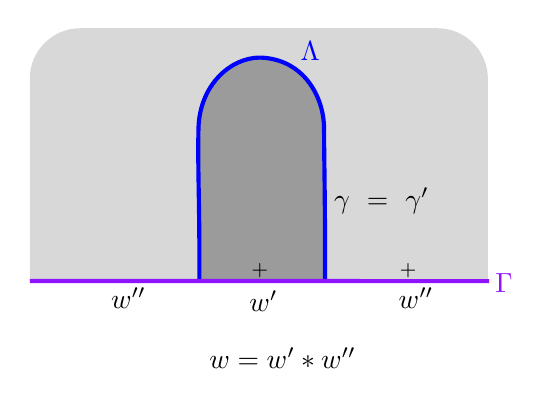
\begin{tikzpicture}[x=0.55pt,y=0.55pt,yscale=-1,xscale=1]
%uncomment if require: \path (0,300); %set diagram left start at 0, and has height of 300

%Rounded Same Side Corner Rect [id:dp4857647198925792] 
\draw  [draw opacity=0][fill={rgb, 255:red, 216; green, 216; blue, 216 }  ,fill opacity=1 ] (147.79,66.7) .. controls (147.79,48.36) and (162.66,33.48) .. (181,33.48) -- (415.57,33.48) .. controls (433.91,33.48) and (448.79,48.36) .. (448.79,66.7) -- (448.79,199.57) .. controls (448.79,199.57) and (448.79,199.57) .. (448.79,199.57) -- (147.79,199.57) .. controls (147.79,199.57) and (147.79,199.57) .. (147.79,199.57) -- cycle ;
%Rounded Same Side Corner Rect [id:dp0653413152711041] 
\draw  [draw opacity=0][fill={rgb, 255:red, 155; green, 155; blue, 155 }  ,fill opacity=1 ] (259.06,93.62) .. controls (259.06,71.05) and (277.36,52.76) .. (299.92,52.76) -- (299.92,52.76) .. controls (322.49,52.76) and (340.79,71.05) .. (340.79,93.62) -- (340.79,198.67) .. controls (340.79,198.67) and (340.79,198.67) .. (340.79,198.67) -- (259.06,198.67) .. controls (259.06,198.67) and (259.06,198.67) .. (259.06,198.67) -- cycle ;
%Curve Lines [id:da750155532713975] 
\draw [color={rgb, 255:red, 0; green, 0; blue, 255 }  ,draw opacity=1 ][line width=1.5]    (259.22,198.61) .. controls (259.47,148.54) and (258.07,128.25) .. (258.63,99.54) .. controls (259.2,70.83) and (279.79,52.67) .. (299.18,52.76) ;
%Curve Lines [id:da8707681237493543] 
\draw [color={rgb, 255:red, 0; green, 0; blue, 255 }  ,draw opacity=1 ][line width=1.5]    (341.73,198.61) .. controls (341.98,148.54) and (341.15,120.54) .. (341.15,99.54) .. controls (341.15,78.54) and (327.79,53.67) .. (299.18,52.76) ;
%Straight Lines [id:da2035266843869472] 
\draw [color={rgb, 255:red, 144; green, 19; blue, 254 }  ,draw opacity=1 ][line width=1.5]    (147.79,199.57) -- (449.65,199.61) ;

% Text Node
\draw (264,241.4) node [anchor=north west][inner sep=0.75pt]    {$w=w'*w''$};
% Text Node
\draw (291.72,186.4) node [anchor=north west][inner sep=0.75pt]  [font=\scriptsize]  {$+$};
% Text Node
\draw (389.07,186.4) node [anchor=north west][inner sep=0.75pt]  [font=\scriptsize]  {$+$};
% Text Node
\draw (290.39,204.4) node [anchor=north west][inner sep=0.75pt]    {$w'$};
% Text Node
\draw (388.49,202.4) node [anchor=north west][inner sep=0.75pt]    {$w''$};
% Text Node
\draw (451.91,193.01) node [anchor=north west][inner sep=0.75pt]  [color={rgb, 255:red, 144; green, 19; blue, 254 }  ,opacity=1 ]  {$\Gamma $};
% Text Node
\draw (323.99,40.4) node [anchor=north west][inner sep=0.75pt]  [color={rgb, 255:red, 0; green, 0; blue, 255 }  ,opacity=1 ]  {$\Lambda $};
% Text Node
\draw (199.49,202.4) node [anchor=north west][inner sep=0.75pt]    {$w''$};
% Text Node
\draw (346,136.4) node [anchor=north west][inner sep=0.75pt]    {$\gamma \ =\ \gamma '$};


\end{tikzpicture}

    \caption{Generic configuration of disks counted in $\Phi_+(w')\Phi_+(w'')$ for a closed Reeb orbit $w$, where neither disk has a nontrivial negative end.}
    \label{fig:hypertight 3}
    \end{minipage}
\end{figure}

 

\begin{example}
    Consider the standard unknot in \Cref{fig:S2xI}. Here, $\Sigma = S^2$ and $\Gamma$ is the equator. Clearly $\xi$ is not hypertight, as $\Gamma$ itself is a contractible Reeb orbit. We compute that $\Phi_+(a*b)=1$, $\Phi_+(a)=1$ and $\Phi_+(b)=1$, so 
    \[\partial_+\circ\Phi_+(a*b)=0 \neq 1 =\Phi_+\circ\partial_\Gamma(a*b). \] So $\Phi_+$ is not
    a chain map. 
\end{example}

\begin{figure}[h]
    \centering
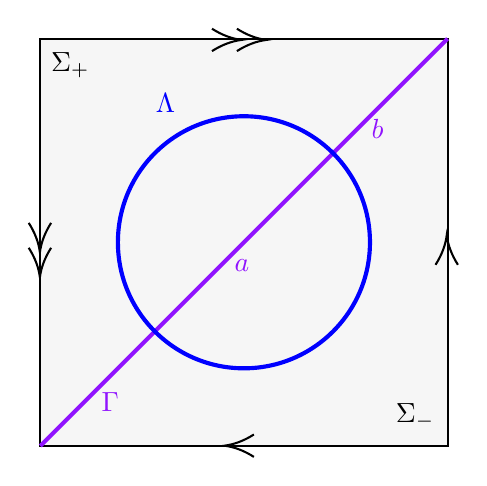
\begin{tikzpicture}[x=0.75pt,y=0.75pt,yscale=-1,xscale=1]
%uncomment if require: \path (0,300); %set diagram left start at 0, and has height of 300

%Shape: Square [id:dp8142439395932848] 
\draw  [fill={rgb, 255:red, 246; green, 246; blue, 246 }  ,fill opacity=1 ] [line width=0.75]  (194.59,51) -- (390.79,51) -- (390.79,247.19) -- (194.59,247.19) -- cycle ;
%Straight Lines [id:da6674803744713234] 
\draw [color={rgb, 255:red, 144; green, 19; blue, 254 }  ,draw opacity=1 ][line width=1.5]    (194.59,247.19) -- (390.79,51) ;
%Shape: Circle [id:dp4532114335600246] 
\draw  [color={rgb, 255:red, 0; green, 0; blue, 255 }  ,draw opacity=1 ][line width=1.5]  (231.97,149.1) .. controls (231.97,115.56) and (259.15,88.37) .. (292.69,88.37) .. controls (326.23,88.37) and (353.41,115.56) .. (353.41,149.1) .. controls (353.41,182.63) and (326.23,209.82) .. (292.69,209.82) .. controls (259.15,209.82) and (231.97,182.63) .. (231.97,149.1) -- cycle ;
\draw  [line width=0.75]  (297.49,252.49) .. controls (292.76,249.49) and (288.03,247.69) .. (283.3,247.1) .. controls (288.03,246.49) and (292.76,244.7) .. (297.49,241.7) ;
\draw  [line width=0.75]  (385,159.94) .. controls (388,155.21) and (389.8,150.48) .. (390.39,145.75) .. controls (391,150.48) and (392.79,155.21) .. (395.79,159.94) ;
\draw  [color={rgb, 255:red, 0; green, 0; blue, 0 }  ,draw opacity=1 ][line width=0.75]  (277.3,46.2) .. controls (282.03,49.2) and (286.76,51) .. (291.49,51.6) .. controls (286.76,52.2) and (282.03,53.99) .. (277.3,56.99) ;
\draw  [color={rgb, 255:red, 0; green, 0; blue, 0 }  ,draw opacity=1 ][line width=0.75]  (289.3,46.2) .. controls (294.03,49.2) and (298.76,51) .. (303.49,51.6) .. controls (298.76,52.2) and (294.03,53.99) .. (289.3,56.99) ;

\draw  [color={rgb, 255:red, 0; green, 0; blue, 0 }  ,draw opacity=1 ][line width=0.75]  (199.79,139.75) .. controls (196.79,144.48) and (194.99,149.21) .. (194.39,153.94) .. controls (193.79,149.21) and (192,144.48) .. (189,139.75) ;
\draw  [color={rgb, 255:red, 0; green, 0; blue, 0 }  ,draw opacity=1 ][line width=0.75]  (199.79,151.75) .. controls (196.79,156.48) and (194.99,161.21) .. (194.39,165.94) .. controls (193.79,161.21) and (192,156.48) .. (189,151.75) ;


% Text Node
\draw (287,156.4) node [anchor=north west][inner sep=0.75pt]  [color={rgb, 255:red, 144; green, 19; blue, 254 }  ,opacity=1 ]  {$a$};
% Text Node
\draw (353,88.4) node [anchor=north west][inner sep=0.75pt]  [color={rgb, 255:red, 144; green, 19; blue, 254 }  ,opacity=1 ]  {$b$};
% Text Node
\draw (222.91,220.01) node [anchor=north west][inner sep=0.75pt]  [color={rgb, 255:red, 144; green, 19; blue, 254 }  ,opacity=1 ]  {$\Gamma $};
% Text Node
\draw (248.99,76.4) node [anchor=north west][inner sep=0.75pt]  [color={rgb, 255:red, 0; green, 0; blue, 255 }  ,opacity=1 ]  {$\Lambda $};
% Text Node
\draw (198.59,56.4) node [anchor=north west][inner sep=0.75pt]    {$\Sigma _{+}$};
% Text Node
\draw (364.59,225.4) node [anchor=north west][inner sep=0.75pt]    {$\Sigma _{-}$};


\end{tikzpicture}

    \caption{Standard Legendrian unknot in $S^2$.}
    \label{fig:S2xI}
\end{figure}
\end{remark}

\begin{proposition}\label{prop:phipmDGA} 
	$\Phi_{\pm}$ are DGA maps.
\end{proposition}

\begin{proof}
    It suffices to show that $\Phi_+$ is a DGA map, as the proof for $\Phi_-$ is identical. We already saw in \Cref{cor:phipmgrading} that $\Phi_+$ preserves the grading. Let $w\in \mathcal{A}_\Gamma$ be a generator, which we think of as a concatenation of some nonempty compatible set of indecomposable Reeb chords. We'd like to show that 
    \[\partial_+\circ \Phi_+(w) = \Phi_+\circ \partial_\Gamma (w).\tag{\dag}\]

    Suppose that $v\in \mathcal{A}_+$ is some monomial appearing in the right hand side of $(\dag)$. Then the coefficient associated to $v$ counts the number of disks of the form in \Cref{fig:decomp 1}. That is, it is a count of two disks with common boundary $\gamma$ whose concatenation has positive end $w$ and negative end $v$. Without loss of generality, we assume that $a$ is a negatively asymptotic endpoint of the disk with positive end $w'$. We also assume for now that the beginning point of $w'$ is distinct from the end point of $w''$. We will address the case that they coincide in \Cref{rem: why hypertight}.

    \begin{figure}[h]
        \centering
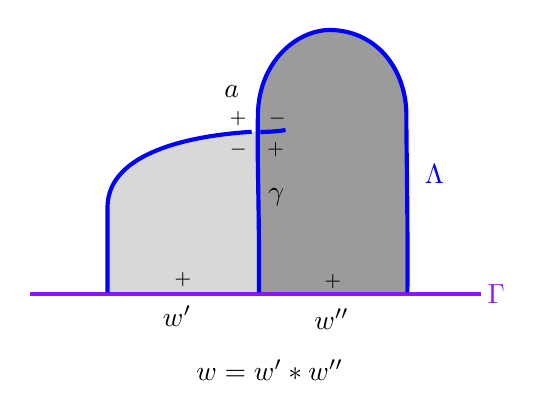
\begin{tikzpicture}[x=0.65pt,y=0.65pt,yscale=-1,xscale=1]
%uncomment if require: \path (0,300); %set diagram left start at 0, and has height of 300

%Shape: Polygon Curved [id:ds753335855235285] 
\draw  [draw opacity=0][fill={rgb, 255:red, 216; green, 216; blue, 216 }  ,fill opacity=1 ] (254.63,127.77) .. controls (274.63,112.77) and (307.63,108.77) .. (326.97,109.54) .. controls (324.79,140.67) and (324.79,173.67) .. (326.79,198.67) .. controls (303.63,200.77) and (273.63,199.77) .. (242.02,198.6) .. controls (241.63,159.77) and (237.63,140.77) .. (254.63,127.77) -- cycle ;
%Rounded Same Side Corner Rect [id:dp7860385290625452] 
\draw  [draw opacity=0][fill={rgb, 255:red, 155; green, 155; blue, 155 }  ,fill opacity=1 ] (326.79,93.26) .. controls (326.79,70.89) and (344.92,52.76) .. (367.29,52.76) -- (367.29,52.76) .. controls (389.65,52.76) and (407.79,70.89) .. (407.79,93.26) -- (407.79,198.67) .. controls (407.79,198.67) and (407.79,198.67) .. (407.79,198.67) -- (326.79,198.67) .. controls (326.79,198.67) and (326.79,198.67) .. (326.79,198.67) -- cycle ;
%Straight Lines [id:da9584533152492841] 
\draw [color={rgb, 255:red, 144; green, 19; blue, 254 }  ,draw opacity=1 ][line width=1.5]    (198.79,199.61) -- (449.65,199.61) ;
%Curve Lines [id:da946107811541346] 
\draw [color={rgb, 255:red, 0; green, 0; blue, 255 }  ,draw opacity=1 ][line width=1.5]    (326.22,198.61) .. controls (326.47,148.54) and (325.07,128.25) .. (325.63,99.54) .. controls (326.2,70.83) and (346.79,52.67) .. (366.18,52.76) ;
%Curve Lines [id:da8141152722043826] 
\draw [color={rgb, 255:red, 0; green, 0; blue, 255 }  ,draw opacity=1 ][line width=1.5]    (408.73,198.61) .. controls (408.98,148.54) and (408.15,120.54) .. (408.15,99.54) .. controls (408.15,78.54) and (394.79,53.67) .. (366.18,52.76) ;
%Curve Lines [id:da5445446606814309] 
\draw [color={rgb, 255:red, 0; green, 0; blue, 255 }  ,draw opacity=1 ][line width=1.5]    (242.02,198.6) .. controls (242.02,177.6) and (242.02,157.6) .. (242.02,150.6) .. controls (242.86,120.6) and (288.82,111.41) .. (322.16,109.41) ;
%Curve Lines [id:da5537871835956659] 
\draw [color={rgb, 255:red, 0; green, 0; blue, 255 }  ,draw opacity=1 ][line width=1.5]    (326.97,109.54) .. controls (330.16,109.41) and (335.16,109.41) .. (340.99,108.41) ;

% Text Node
\draw (290,234.4) node [anchor=north west][inner sep=0.75pt]    {$w=w'*w''$};
% Text Node
\draw (330,139.4) node [anchor=north west][inner sep=0.75pt]    {$\gamma $};
% Text Node
\draw (277.72,186.4) node [anchor=north west][inner sep=0.75pt]  [font=\scriptsize]  {$+$};
% Text Node
\draw (361.07,187.4) node [anchor=north west][inner sep=0.75pt]  [font=\scriptsize]  {$+$};
% Text Node
\draw (329.24,113.81) node [anchor=north west][inner sep=0.75pt]  [font=\scriptsize]  {$+$};
% Text Node
\draw (308.41,96.81) node [anchor=north west][inner sep=0.75pt]  [font=\scriptsize]  {$+$};
% Text Node
\draw (308.41,113.81) node [anchor=north west][inner sep=0.75pt]  [font=\scriptsize]  {$-$};
% Text Node
\draw (305.56,82.4) node [anchor=north west][inner sep=0.75pt]    {$a$};
% Text Node
\draw (271.39,204.4) node [anchor=north west][inner sep=0.75pt]    {$w'$};
% Text Node
\draw (355.49,206.4) node [anchor=north west][inner sep=0.75pt]    {$w''$};
% Text Node
\draw (451.91,193.01) node [anchor=north west][inner sep=0.75pt]  [color={rgb, 255:red, 144; green, 19; blue, 254 }  ,opacity=1 ]  {$\Gamma $};
% Text Node
\draw (416.99,126.4) node [anchor=north west][inner sep=0.75pt]  [color={rgb, 255:red, 0; green, 0; blue, 255 }  ,opacity=1 ]  {$\Lambda $};
% Text Node
\draw (330.07,96.81) node [anchor=north west][inner sep=0.75pt]  [font=\scriptsize]  {$-$};


\end{tikzpicture}

        \caption{A collection of disks corresponding to $v$ in $\Phi_+\circ \partial_\Gamma$.}
        \label{fig:decomp 1}
    \end{figure}

We'd like to show that $v$ appears as a monomial on the right hand side with the same $\Z_2$ coefficient as on the left hand side of $(\dag)$. Notice that concatenating the two disks along their common boundary $\gamma$ produces a disk with a positive end at $w'*w'' = w$, one obtuse corner negatively asymptotic to some $a\in \mathcal{A}_+$, and all other corners acute and negatively asymptotic to chords in $\mathcal{A}_+$. We may then consider the disks in \Cref{fig:decomp 1} as a degeneration of such a disk. Degenerating along the other strand produces the configuration in \Cref{fig:decomp 2}.


    \begin{figure}[h]
        \centering
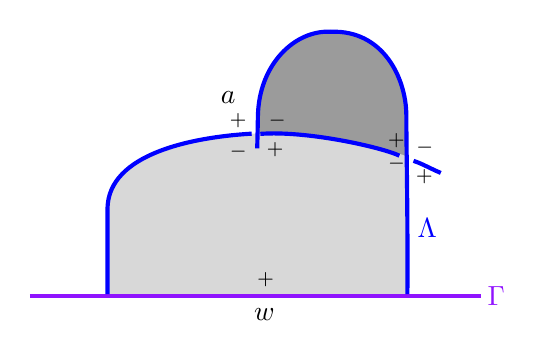
\begin{tikzpicture}[x=0.65pt,y=0.65pt,yscale=-1,xscale=1]
%uncomment if require: \path (0,300); %set diagram left start at 0, and has height of 300

%Rounded Same Side Corner Rect [id:dp7283622528316729] 
\draw  [draw opacity=0][fill={rgb, 255:red, 155; green, 155; blue, 155 }  ,fill opacity=1 ] (317.28,107.44) .. controls (317.28,85.07) and (335.41,66.94) .. (357.78,66.94) -- (357.78,66.94) .. controls (380.15,66.94) and (398.28,85.07) .. (398.28,107.44) -- (398.28,212.85) .. controls (398.28,212.85) and (398.28,212.85) .. (398.28,212.85) -- (317.28,212.85) .. controls (317.28,212.85) and (317.28,212.85) .. (317.28,212.85) -- cycle ;
%Shape: Polygon Curved [id:ds5624747002426606] 
\draw  [draw opacity=0][fill={rgb, 255:red, 216; green, 216; blue, 216 }  ,fill opacity=1 ] (245.63,142.01) .. controls (265.63,127.01) and (298.63,123.01) .. (317.97,123.78) .. controls (335.51,122.5) and (375.51,127.5) .. (398.28,135.87) .. controls (399.51,153.5) and (399.8,163.64) .. (399.79,171.28) .. controls (399.77,178.91) and (399.51,192.5) .. (399.73,212.85) .. controls (370.51,214.5) and (329.94,213.44) .. (315.22,213.85) .. controls (292.51,213.5) and (264.63,214.01) .. (233.02,212.84) .. controls (232.63,174.01) and (228.63,155.01) .. (245.63,142.01) -- cycle ;
%Straight Lines [id:da056931289631659165] 
\draw [color={rgb, 255:red, 144; green, 19; blue, 254 }  ,draw opacity=1 ][line width=1.5]    (189.79,213.85) -- (440.65,213.85) ;
%Curve Lines [id:da3040989568987509] 
\draw [color={rgb, 255:red, 0; green, 0; blue, 255 }  ,draw opacity=1 ][line width=1.5]    (316.28,131.87) .. controls (316.28,124.87) and (316.07,142.49) .. (316.63,113.78) .. controls (317.2,85.07) and (337.21,65.89) .. (357.18,67) ;
%Curve Lines [id:da5173352679778818] 
\draw [color={rgb, 255:red, 0; green, 0; blue, 255 }  ,draw opacity=1 ][line width=1.5]    (399.73,212.85) .. controls (399.98,162.78) and (399.15,134.78) .. (399.15,113.78) .. controls (399.15,92.78) and (386.21,65.89) .. (357.18,67) ;
%Curve Lines [id:da9555803111220733] 
\draw [color={rgb, 255:red, 0; green, 0; blue, 255 }  ,draw opacity=1 ][line width=1.5]    (233.02,212.84) .. controls (233.02,191.84) and (233.02,171.84) .. (233.02,164.84) .. controls (233.86,134.84) and (279.82,125.65) .. (313.16,123.65) ;
%Curve Lines [id:da21421412371935877] 
\draw [color={rgb, 255:red, 0; green, 0; blue, 255 }  ,draw opacity=1 ][line width=1.5]    (317.97,123.78) .. controls (343.28,121.87) and (384.28,130.87) .. (395.28,135.87) ;
%Curve Lines [id:da4487145818426833] 
\draw [color={rgb, 255:red, 0; green, 0; blue, 255 }  ,draw opacity=1 ][line width=1.5]    (403.14,138.78) .. controls (408.28,140.48) and (411.28,142.48) .. (418.28,145.48) ;

% Text Node
\draw (313,219.64) node [anchor=north west][inner sep=0.75pt]    {$w$};
% Text Node
\draw (314.72,199.64) node [anchor=north west][inner sep=0.75pt]  [font=\scriptsize]  {$+$};
% Text Node
\draw (319.97,127.18) node [anchor=north west][inner sep=0.75pt]  [font=\scriptsize]  {$+$};
% Text Node
\draw (299.41,111.05) node [anchor=north west][inner sep=0.75pt]  [font=\scriptsize]  {$+$};
% Text Node
\draw (299.41,128.05) node [anchor=north west][inner sep=0.75pt]  [font=\scriptsize]  {$-$};
% Text Node
\draw (294.56,98.64) node [anchor=north west][inner sep=0.75pt]    {$a$};
% Text Node
\draw (442.91,207.25) node [anchor=north west][inner sep=0.75pt]  [color={rgb, 255:red, 144; green, 19; blue, 254 }  ,opacity=1 ]  {$\Gamma $};
% Text Node
\draw (403.99,169.64) node [anchor=north west][inner sep=0.75pt]  [color={rgb, 255:red, 0; green, 0; blue, 255 }  ,opacity=1 ]  {$\Lambda $};
% Text Node
\draw (321.07,111.05) node [anchor=north west][inner sep=0.75pt]  [font=\scriptsize]  {$-$};
% Text Node
\draw (402.97,142.18) node [anchor=north west][inner sep=0.75pt]  [font=\scriptsize]  {$+$};
% Text Node
\draw (387.41,122.05) node [anchor=north west][inner sep=0.75pt]  [font=\scriptsize]  {$+$};
% Text Node
\draw (387.41,135.05) node [anchor=north west][inner sep=0.75pt]  [font=\scriptsize]  {$-$};
% Text Node
\draw (403.07,126.05) node [anchor=north west][inner sep=0.75pt]  [font=\scriptsize]  {$-$};


\end{tikzpicture}

        \caption{Degeneration of disk along second strand, corresponding to $v$ in $\partial_+\circ \Phi_+$. }
        \label{fig:decomp 2}
    \end{figure}

    These disks contribute $+1$ to the coefficient of $v$ in the left hand side of $(\dag)$.  Note that we assumed a particular position of the Legendrian knot relative to the dividing set $\Gamma$. In particular, we assumed that one strand at $a$ intersects $\Gamma$, and the other intersects $\Lambda$.  In the event that the knot $\Lambda$ is not in this position, then without loss of generality $\Lambda$ must occupy one of the other three configurations in \Cref{fig:decomp 3}. In each of these cases, following a similar degeneration argument along each strand would contribute $2\equiv 0$ (mod $2$) to either the left hand side or right hand side of $(\dag)$. 

    \begin{figure}[h]
        \centering
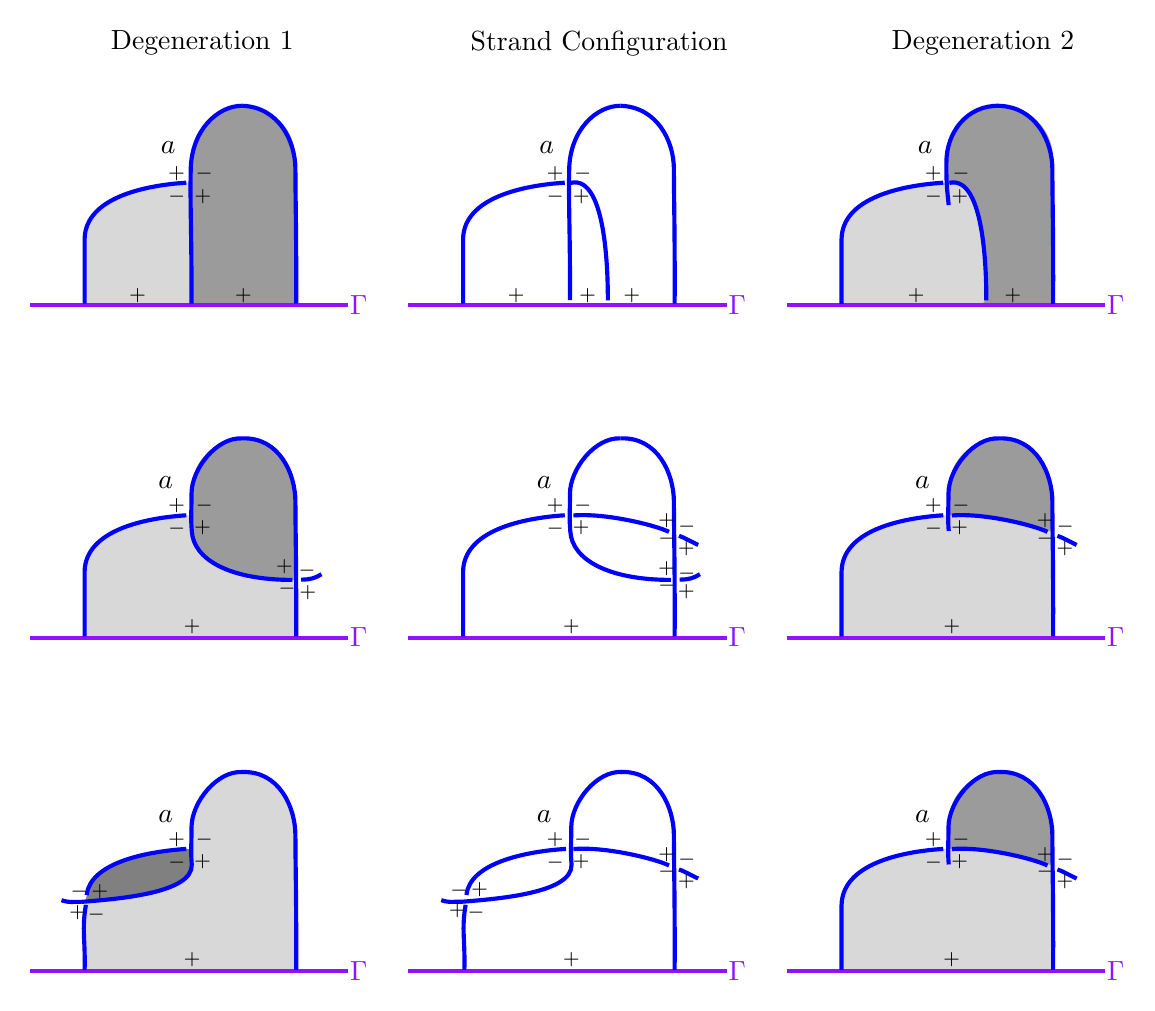
\begin{tikzpicture}[x=0.65pt,y=0.65pt,yscale=-1,xscale=1]
%uncomment if require: \path (0,736); %set diagram left start at 0, and has height of 736

%Rounded Same Side Corner Rect [id:dp8478641795641755] 
\draw  [draw opacity=0][fill={rgb, 255:red, 155; green, 155; blue, 155 }  ,fill opacity=1 ] (526.91,95.25) .. controls (526.91,78.87) and (540.19,65.59) .. (556.57,65.59) -- (556.57,65.59) .. controls (572.95,65.59) and (586.23,78.87) .. (586.23,95.25) -- (586.23,175.68) .. controls (586.23,175.68) and (586.23,175.68) .. (586.23,175.68) -- (526.91,175.68) .. controls (526.91,175.68) and (526.91,175.68) .. (526.91,175.68) -- cycle ;
%Shape: Polygon Curved [id:ds4220399586461909] 
\draw  [draw opacity=0][fill={rgb, 255:red, 216; green, 216; blue, 216 }  ,fill opacity=1 ] (477.52,122.24) .. controls (491.63,110.92) and (514.91,107.9) .. (528.55,108.48) .. controls (542.2,106.54) and (547.15,133.03) .. (547.14,148.04) .. controls (549.25,180.48) and (553.48,176.71) .. (528.42,175.73) .. controls (512.09,177.32) and (490.92,176.56) .. (468.63,175.68) .. controls (468.35,146.38) and (465.52,132.04) .. (477.52,122.24) -- cycle ;
%Straight Lines [id:da01700147304836741] 
\draw [color={rgb, 255:red, 144; green, 19; blue, 254 }  ,draw opacity=1 ][line width=1.5]    (438.12,176.44) -- (615.1,176.44) ;
%Curve Lines [id:da9073821902766053] 
\draw [color={rgb, 255:red, 0; green, 0; blue, 255 }  ,draw opacity=1 ][line width=1.5]    (528.17,120.82) .. controls (527.46,113.28) and (526.76,109.51) .. (526.91,97.32) .. controls (526.76,80.08) and (538.67,65.17) .. (556.22,65.63) ;
%Curve Lines [id:da020791996857834505] 
\draw [color={rgb, 255:red, 0; green, 0; blue, 255 }  ,draw opacity=1 ][line width=1.5]    (586.23,175.68) .. controls (586.41,137.91) and (585.82,116.78) .. (585.82,100.93) .. controls (585.82,85.09) and (576.4,66.32) .. (556.22,65.63) ;
%Curve Lines [id:da9367721093741916] 
\draw [color={rgb, 255:red, 0; green, 0; blue, 255 }  ,draw opacity=1 ][line width=1.5]    (468.63,175.68) .. controls (468.63,159.83) and (468.63,144.74) .. (468.63,139.46) .. controls (469.21,116.82) and (501.64,109.89) .. (525.16,108.38) ;
%Curve Lines [id:da15003571515645708] 
\draw [color={rgb, 255:red, 0; green, 0; blue, 255 }  ,draw opacity=1 ][line width=1.5]    (528.55,108.48) .. controls (549.1,103.69) and (549.1,164.05) .. (549.1,173.86) ;
%Straight Lines [id:da365306346273397] 
\draw [color={rgb, 255:red, 144; green, 19; blue, 254 }  ,draw opacity=1 ][line width=1.5]    (227.72,176.42) -- (404.7,176.42) ;
%Curve Lines [id:da008177810442077105] 
\draw [color={rgb, 255:red, 0; green, 0; blue, 255 }  ,draw opacity=1 ][line width=1.5]    (317.62,173.66) .. controls (317.8,135.88) and (316.81,122.57) .. (317.21,100.91) .. controls (317.61,79.25) and (332.13,65.55) .. (345.82,65.61) ;
%Curve Lines [id:da7403735975285] 
\draw [color={rgb, 255:red, 0; green, 0; blue, 255 }  ,draw opacity=1 ][line width=1.5]    (375.83,175.66) .. controls (376.01,137.88) and (375.42,116.76) .. (375.42,100.91) .. controls (375.42,85.07) and (365.99,66.3) .. (345.82,65.61) ;
%Curve Lines [id:da0662834269046726] 
\draw [color={rgb, 255:red, 0; green, 0; blue, 255 }  ,draw opacity=1 ][line width=1.5]    (258.22,175.65) .. controls (258.22,159.81) and (258.22,144.72) .. (258.22,139.44) .. controls (258.81,116.8) and (291.24,109.87) .. (314.75,108.36) ;
%Curve Lines [id:da7433657735591765] 
\draw [color={rgb, 255:red, 0; green, 0; blue, 255 }  ,draw opacity=1 ][line width=1.5]    (318.15,108.46) .. controls (338.7,103.67) and (338.7,164.03) .. (338.7,173.84) ;
%Shape: Polygon Curved [id:ds31680982092206333] 
\draw  [draw opacity=0][fill={rgb, 255:red, 216; green, 216; blue, 216 }  ,fill opacity=1 ] (56.71,122.21) .. controls (70.82,110.89) and (94.1,107.88) .. (107.75,108.46) .. controls (106.21,131.95) and (106.21,156.84) .. (107.62,175.71) .. controls (91.28,177.29) and (70.12,176.54) .. (47.82,175.65) .. controls (47.54,146.36) and (44.72,132.02) .. (56.71,122.21) -- cycle ;
%Rounded Same Side Corner Rect [id:dp7873858136027139] 
\draw  [draw opacity=0][fill={rgb, 255:red, 155; green, 155; blue, 155 }  ,fill opacity=1 ] (107.62,94.18) .. controls (107.62,78.4) and (120.41,65.61) .. (136.19,65.61) -- (136.19,65.61) .. controls (151.97,65.61) and (164.76,78.4) .. (164.76,94.18) -- (164.76,175.71) .. controls (164.76,175.71) and (164.76,175.71) .. (164.76,175.71) -- (107.62,175.71) .. controls (107.62,175.71) and (107.62,175.71) .. (107.62,175.71) -- cycle ;
%Straight Lines [id:da5691303057731534] 
\draw [color={rgb, 255:red, 144; green, 19; blue, 254 }  ,draw opacity=1 ][line width=1.5]    (17.32,176.42) -- (194.3,176.42) ;
%Curve Lines [id:da3555027261073602] 
\draw [color={rgb, 255:red, 0; green, 0; blue, 255 }  ,draw opacity=1 ][line width=1.5]    (107.22,175.66) .. controls (107.39,137.88) and (106.4,122.57) .. (106.81,100.91) .. controls (107.21,79.25) and (121.73,65.55) .. (135.41,65.61) ;
%Curve Lines [id:da8276958583505334] 
\draw [color={rgb, 255:red, 0; green, 0; blue, 255 }  ,draw opacity=1 ][line width=1.5]    (165.43,175.66) .. controls (165.6,137.88) and (165.01,116.76) .. (165.01,100.91) .. controls (165.01,85.07) and (155.59,66.3) .. (135.41,65.61) ;
%Curve Lines [id:da883957554896516] 
\draw [color={rgb, 255:red, 0; green, 0; blue, 255 }  ,draw opacity=1 ][line width=1.5]    (47.82,175.65) .. controls (47.82,159.81) and (47.82,144.72) .. (47.82,139.44) .. controls (48.41,116.8) and (80.83,109.87) .. (104.35,108.36) ;
%Straight Lines [id:da3817286246594993] 
\draw [color={rgb, 255:red, 144; green, 19; blue, 254 }  ,draw opacity=1 ][line width=1.5]    (227.72,361.32) -- (404.7,361.32) ;
%Curve Lines [id:da19967832934299778] 
\draw [color={rgb, 255:red, 0; green, 0; blue, 255 }  ,draw opacity=1 ][line width=1.5]    (373.75,329.19) .. controls (339.18,329.19) and (318.6,318.05) .. (317.8,301.92) .. controls (317.23,294.14) and (317.58,294.63) .. (317.66,281.03) .. controls (317.74,267.42) and (331.72,249.67) .. (345.82,250.51) ;
%Curve Lines [id:da08453622786858395] 
\draw [color={rgb, 255:red, 0; green, 0; blue, 255 }  ,draw opacity=1 ][line width=1.5]    (375.83,360.56) .. controls (376.01,322.78) and (375.42,301.66) .. (375.42,285.81) .. controls (375.42,269.97) and (366.29,249.67) .. (345.82,250.51) ;
%Curve Lines [id:da34237711425155015] 
\draw [color={rgb, 255:red, 0; green, 0; blue, 255 }  ,draw opacity=1 ][line width=1.5]    (258.22,360.55) .. controls (258.22,344.71) and (258.22,329.62) .. (258.22,324.33) .. controls (258.81,301.7) and (291.24,294.77) .. (314.75,293.26) ;
%Curve Lines [id:da25952637956298763] 
\draw [color={rgb, 255:red, 0; green, 0; blue, 255 }  ,draw opacity=1 ][line width=1.5]    (319.56,293.36) .. controls (337.42,291.91) and (364.93,298.7) .. (372.69,302.48) ;
%Curve Lines [id:da8302557176757372] 
\draw [color={rgb, 255:red, 0; green, 0; blue, 255 }  ,draw opacity=1 ][line width=1.5]    (378.24,304.67) .. controls (381.86,305.95) and (383.98,307.46) .. (388.92,309.73) ;
%Curve Lines [id:da4688076893662383] 
\draw [color={rgb, 255:red, 0; green, 0; blue, 255 }  ,draw opacity=1 ][line width=1.5]    (378.62,329.02) .. controls (383.56,329.02) and (386.38,328.27) .. (389.9,326) ;
%Rounded Same Side Corner Rect [id:dp5368336638655509] 
\draw  [draw opacity=0][fill={rgb, 255:red, 155; green, 155; blue, 155 }  ,fill opacity=1 ] (528.07,279.05) .. controls (528.07,263.27) and (540.86,250.47) .. (556.64,250.47) -- (556.64,250.47) .. controls (572.42,250.47) and (585.21,263.27) .. (585.21,279.05) -- (585.21,360.57) .. controls (585.21,360.57) and (585.21,360.57) .. (585.21,360.57) -- (528.07,360.57) .. controls (528.07,360.57) and (528.07,360.57) .. (528.07,360.57) -- cycle ;
%Shape: Polygon Curved [id:ds7259707808459595] 
\draw  [draw opacity=0][fill={rgb, 255:red, 216; green, 216; blue, 216 }  ,fill opacity=1 ] (477.52,307.12) .. controls (491.63,295.8) and (514.91,292.78) .. (528.55,293.36) .. controls (540.93,292.4) and (569.15,296.17) .. (585.21,302.48) .. controls (586.08,315.79) and (586.28,323.44) .. (586.27,329.2) .. controls (586.26,334.96) and (586.08,345.21) .. (586.23,360.57) .. controls (565.62,361.81) and (537,361.01) .. (526.61,361.32) .. controls (510.59,361.06) and (490.92,361.45) .. (468.63,360.56) .. controls (468.35,331.27) and (465.52,316.93) .. (477.52,307.12) -- cycle ;
%Straight Lines [id:da6706317193353153] 
\draw [color={rgb, 255:red, 144; green, 19; blue, 254 }  ,draw opacity=1 ][line width=1.5]    (438.12,361.32) -- (615.1,361.32) ;
%Curve Lines [id:da27162365242580266] 
\draw [color={rgb, 255:red, 0; green, 0; blue, 255 }  ,draw opacity=1 ][line width=1.5]    (528.2,301.93) .. controls (527.63,294.15) and (527.98,294.64) .. (528.07,281.03) .. controls (528.15,267.43) and (542.12,249.68) .. (556.22,250.52) ;
%Curve Lines [id:da05700777505965493] 
\draw [color={rgb, 255:red, 0; green, 0; blue, 255 }  ,draw opacity=1 ][line width=1.5]    (586.23,360.57) .. controls (586.41,322.79) and (585.82,301.66) .. (585.82,285.82) .. controls (585.82,269.97) and (576.69,249.68) .. (556.22,250.52) ;
%Curve Lines [id:da8291356113389969] 
\draw [color={rgb, 255:red, 0; green, 0; blue, 255 }  ,draw opacity=1 ][line width=1.5]    (468.63,360.56) .. controls (468.63,344.72) and (468.63,329.62) .. (468.63,324.34) .. controls (469.21,301.71) and (501.64,294.77) .. (525.16,293.27) ;
%Curve Lines [id:da02708600284906093] 
\draw [color={rgb, 255:red, 0; green, 0; blue, 255 }  ,draw opacity=1 ][line width=1.5]    (529.96,293.36) .. controls (547.82,291.92) and (575.33,298.71) .. (583.09,302.48) ;
%Curve Lines [id:da35155374338891043] 
\draw [color={rgb, 255:red, 0; green, 0; blue, 255 }  ,draw opacity=1 ][line width=1.5]    (588.64,304.68) .. controls (592.27,305.96) and (594.38,307.47) .. (599.32,309.73) ;
%Rounded Same Side Corner Rect [id:dp8807575702948518] 
\draw  [draw opacity=0][fill={rgb, 255:red, 155; green, 155; blue, 155 }  ,fill opacity=1 ] (107.26,279.17) .. controls (107.26,263.32) and (120.11,250.47) .. (135.96,250.47) -- (135.96,250.47) .. controls (151.8,250.47) and (164.65,263.32) .. (164.65,279.17) -- (164.65,360.57) .. controls (164.65,360.57) and (164.65,360.57) .. (164.65,360.57) -- (107.26,360.57) .. controls (107.26,360.57) and (107.26,360.57) .. (107.26,360.57) -- cycle ;
%Shape: Polygon Curved [id:ds19007577708356416] 
\draw  [draw opacity=0][fill={rgb, 255:red, 216; green, 216; blue, 216 }  ,fill opacity=1 ] (56.71,307.12) .. controls (70.82,295.8) and (94.1,292.78) .. (107.75,293.36) .. controls (105.39,308.85) and (113.86,320.93) .. (130.79,325.45) .. controls (147.72,329.23) and (157.6,329.98) .. (165.47,329.2) .. controls (165.46,334.96) and (165.27,345.21) .. (165.43,360.57) .. controls (144.81,361.81) and (116.2,361.01) .. (105.81,361.32) .. controls (89.79,361.06) and (70.12,361.45) .. (47.82,360.56) .. controls (47.54,331.27) and (44.72,316.93) .. (56.71,307.12) -- cycle ;
%Straight Lines [id:da39287635183877834] 
\draw [color={rgb, 255:red, 144; green, 19; blue, 254 }  ,draw opacity=1 ][line width=1.5]    (17.32,361.32) -- (194.3,361.32) ;
%Curve Lines [id:da6195270766661212] 
\draw [color={rgb, 255:red, 0; green, 0; blue, 255 }  ,draw opacity=1 ][line width=1.5]    (163.35,329.2) .. controls (128.78,329.2) and (108.2,318.06) .. (107.4,301.93) .. controls (106.83,294.15) and (107.18,294.64) .. (107.26,281.03) .. controls (107.34,267.43) and (121.32,249.68) .. (135.41,250.52) ;
%Curve Lines [id:da19457611989691004] 
\draw [color={rgb, 255:red, 0; green, 0; blue, 255 }  ,draw opacity=1 ][line width=1.5]    (165.43,360.57) .. controls (165.6,322.79) and (165.01,301.66) .. (165.01,285.82) .. controls (165.01,269.97) and (155.89,249.68) .. (135.41,250.52) ;
%Curve Lines [id:da4342653455582459] 
\draw [color={rgb, 255:red, 0; green, 0; blue, 255 }  ,draw opacity=1 ][line width=1.5]    (47.82,360.56) .. controls (47.82,344.72) and (47.82,329.62) .. (47.82,324.34) .. controls (48.41,301.71) and (80.83,294.77) .. (104.35,293.27) ;
%Curve Lines [id:da2901068029446341] 
\draw [color={rgb, 255:red, 0; green, 0; blue, 255 }  ,draw opacity=1 ][line width=1.5]    (168.21,329.03) .. controls (173.15,329.03) and (175.97,328.27) .. (179.5,326.01) ;
%Shape: Polygon Curved [id:ds8097585381770129] 
\draw  [draw opacity=0][fill={rgb, 255:red, 128; green, 128; blue, 128 }  ,fill opacity=1 ] (48.53,508.32) .. controls (49.22,490.34) and (68.95,487.15) .. (72.46,484.3) .. controls (75.98,481.45) and (89.43,479.02) .. (107.04,478.85) .. controls (109.89,497.88) and (100.82,496.58) .. (88.39,502.24) .. controls (74.38,507.73) and (74.99,510.54) .. (48.53,508.32) -- cycle ;
%Shape: Polygon Curved [id:ds21474796212793756] 
\draw  [draw opacity=0][fill={rgb, 255:red, 216; green, 216; blue, 216 }  ,fill opacity=1 ] (64.77,506.34) .. controls (97.56,500.73) and (107.44,502.24) .. (107.75,478.85) .. controls (102.09,451.1) and (124.8,434.4) .. (135.41,436.01) .. controls (169.82,439.03) and (166.99,480.53) .. (164.41,487.97) .. controls (165.27,501.27) and (165.47,508.93) .. (165.47,514.69) .. controls (165.46,520.45) and (165.27,530.7) .. (165.43,546.06) .. controls (144.81,547.3) and (116.2,546.5) .. (105.81,546.81) .. controls (89.79,546.55) and (70.12,546.93) .. (47.82,546.05) .. controls (47.14,501.06) and (42.9,508.6) .. (64.77,506.34) -- cycle ;
%Straight Lines [id:da2342145155433446] 
\draw [color={rgb, 255:red, 144; green, 19; blue, 254 }  ,draw opacity=1 ][line width=1.5]    (17.32,546.81) -- (194.3,546.81) ;
%Curve Lines [id:da16058065187659798] 
\draw [color={rgb, 255:red, 0; green, 0; blue, 255 }  ,draw opacity=1 ][line width=1.5]    (45.89,508.19) .. controls (65.2,506.64) and (108.2,503.55) .. (107.4,487.41) .. controls (106.83,479.64) and (107.18,480.13) .. (107.26,466.52) .. controls (107.34,452.92) and (121.32,435.17) .. (135.41,436.01) ;
%Curve Lines [id:da506985375263707] 
\draw [color={rgb, 255:red, 0; green, 0; blue, 255 }  ,draw opacity=1 ][line width=1.5]    (165.43,546.06) .. controls (165.6,508.28) and (165.01,487.15) .. (165.01,471.31) .. controls (165.01,455.46) and (155.89,435.17) .. (135.41,436.01) ;
%Curve Lines [id:da4978029539966864] 
\draw [color={rgb, 255:red, 0; green, 0; blue, 255 }  ,draw opacity=1 ][line width=1.5]    (48.98,504.37) .. controls (50.84,486.85) and (80.83,480.26) .. (104.35,478.75) ;
%Curve Lines [id:da9345302663365935] 
\draw [color={rgb, 255:red, 0; green, 0; blue, 255 }  ,draw opacity=1 ][line width=1.5]    (34.97,507.27) .. controls (39.91,508.78) and (39.91,508.02) .. (45.89,508.19) ;
%Curve Lines [id:da7840648111693094] 
\draw [color={rgb, 255:red, 0; green, 0; blue, 255 }  ,draw opacity=1 ][line width=1.5]    (47.82,546.05) .. controls (48.27,528.52) and (46.15,523.99) .. (48.53,509.83) ;
%Straight Lines [id:da43127114159289603] 
\draw [color={rgb, 255:red, 144; green, 19; blue, 254 }  ,draw opacity=1 ][line width=1.5]    (227.72,546.77) -- (404.7,546.77) ;
%Curve Lines [id:da7936200023986313] 
\draw [color={rgb, 255:red, 0; green, 0; blue, 255 }  ,draw opacity=1 ][line width=1.5]    (375.83,546.02) .. controls (376.01,508.24) and (375.42,487.11) .. (375.42,471.27) .. controls (375.42,455.42) and (366.29,435.13) .. (345.82,435.97) ;
%Curve Lines [id:da5553581916733628] 
\draw [color={rgb, 255:red, 0; green, 0; blue, 255 }  ,draw opacity=1 ][line width=1.5]    (319.56,478.81) .. controls (337.42,477.37) and (364.93,484.16) .. (372.69,487.93) ;
%Curve Lines [id:da19309251962109042] 
\draw [color={rgb, 255:red, 0; green, 0; blue, 255 }  ,draw opacity=1 ][line width=1.5]    (378.24,490.13) .. controls (381.86,491.41) and (383.98,492.92) .. (388.92,495.18) ;
%Curve Lines [id:da8818020070774513] 
\draw [color={rgb, 255:red, 0; green, 0; blue, 255 }  ,draw opacity=1 ][line width=1.5]    (257,508.15) .. controls (276.31,506.6) and (319.31,503.51) .. (318.51,487.38) .. controls (317.94,479.6) and (318.29,480.09) .. (318.37,466.48) .. controls (318.45,452.88) and (332.43,435.13) .. (346.52,435.97) ;
%Curve Lines [id:da8844108817791918] 
\draw [color={rgb, 255:red, 0; green, 0; blue, 255 }  ,draw opacity=1 ][line width=1.5]    (260.09,504.34) .. controls (261.95,486.81) and (291.94,480.22) .. (315.46,478.71) ;
%Curve Lines [id:da2089518563167969] 
\draw [color={rgb, 255:red, 0; green, 0; blue, 255 }  ,draw opacity=1 ][line width=1.5]    (246.08,507.23) .. controls (251.02,508.74) and (251.02,507.98) .. (257,508.15) ;
%Curve Lines [id:da5524535600432985] 
\draw [color={rgb, 255:red, 0; green, 0; blue, 255 }  ,draw opacity=1 ][line width=1.5]    (258.93,546.01) .. controls (259.38,528.48) and (257.26,523.95) .. (259.64,509.79) ;
%Rounded Same Side Corner Rect [id:dp9651487703092341] 
\draw  [draw opacity=0][fill={rgb, 255:red, 155; green, 155; blue, 155 }  ,fill opacity=1 ] (528.07,464.5) .. controls (528.07,448.72) and (540.86,435.93) .. (556.64,435.93) -- (556.64,435.93) .. controls (572.42,435.93) and (585.21,448.72) .. (585.21,464.5) -- (585.21,546.03) .. controls (585.21,546.03) and (585.21,546.03) .. (585.21,546.03) -- (528.07,546.03) .. controls (528.07,546.03) and (528.07,546.03) .. (528.07,546.03) -- cycle ;
%Shape: Polygon Curved [id:ds8318132531666931] 
\draw  [draw opacity=0][fill={rgb, 255:red, 216; green, 216; blue, 216 }  ,fill opacity=1 ] (477.52,492.58) .. controls (491.63,481.26) and (514.91,478.24) .. (528.55,478.82) .. controls (540.93,477.85) and (569.15,481.63) .. (585.21,487.94) .. controls (586.08,501.24) and (586.28,508.9) .. (586.27,514.66) .. controls (586.26,520.42) and (586.08,530.67) .. (586.23,546.03) .. controls (565.62,547.27) and (537,546.47) .. (526.61,546.78) .. controls (510.59,546.52) and (490.92,546.9) .. (468.63,546.02) .. controls (468.35,516.72) and (465.52,502.39) .. (477.52,492.58) -- cycle ;
%Straight Lines [id:da5397302702942384] 
\draw [color={rgb, 255:red, 144; green, 19; blue, 254 }  ,draw opacity=1 ][line width=1.5]    (438.12,546.78) -- (615.1,546.78) ;
%Curve Lines [id:da7027722509569354] 
\draw [color={rgb, 255:red, 0; green, 0; blue, 255 }  ,draw opacity=1 ][line width=1.5]    (528.2,487.38) .. controls (527.63,479.6) and (527.98,480.1) .. (528.07,466.49) .. controls (528.15,452.89) and (542.12,435.14) .. (556.22,435.98) ;
%Curve Lines [id:da556862916473045] 
\draw [color={rgb, 255:red, 0; green, 0; blue, 255 }  ,draw opacity=1 ][line width=1.5]    (586.23,546.03) .. controls (586.41,508.25) and (585.82,487.12) .. (585.82,471.27) .. controls (585.82,455.43) and (576.69,435.14) .. (556.22,435.98) ;
%Curve Lines [id:da5531140197973574] 
\draw [color={rgb, 255:red, 0; green, 0; blue, 255 }  ,draw opacity=1 ][line width=1.5]    (468.63,546.02) .. controls (468.63,530.17) and (468.63,515.08) .. (468.63,509.8) .. controls (469.21,487.16) and (501.64,480.23) .. (525.16,478.72) ;
%Curve Lines [id:da08714891474134512] 
\draw [color={rgb, 255:red, 0; green, 0; blue, 255 }  ,draw opacity=1 ][line width=1.5]    (529.96,478.82) .. controls (547.82,477.38) and (575.33,484.17) .. (583.09,487.94) ;
%Curve Lines [id:da28506229220896984] 
\draw [color={rgb, 255:red, 0; green, 0; blue, 255 }  ,draw opacity=1 ][line width=1.5]    (588.64,490.14) .. controls (592.27,491.42) and (594.38,492.93) .. (599.32,495.19) ;

% Text Node
\draw (261,22.5) node [anchor=north west][inner sep=0.75pt]   [align=left] {Strand Configuration};
% Text Node
\draw (61,22.5) node [anchor=north west][inner sep=0.75pt]   [align=left] {Degeneration 1};
% Text Node
\draw (495,22.5) node [anchor=north west][inner sep=0.75pt]   [align=left] {Degeneration 2};
% Text Node
\draw (281.5,165.71) node [anchor=north west][inner sep=0.75pt]  [font=\scriptsize]  {$+$};
% Text Node
\draw (345.94,165.71) node [anchor=north west][inner sep=0.75pt]  [font=\scriptsize]  {$+$};
% Text Node
\draw (317.84,110.55) node [anchor=north west][inner sep=0.75pt]  [font=\scriptsize]  {$+$};
% Text Node
\draw (303.14,97.72) node [anchor=north west][inner sep=0.75pt]  [font=\scriptsize]  {$+$};
% Text Node
\draw (303.14,110.55) node [anchor=north west][inner sep=0.75pt]  [font=\scriptsize]  {$-$};
% Text Node
\draw (299.13,84.11) node [anchor=north west][inner sep=0.75pt]    {$a$};
% Text Node
\draw (404.37,169.57) node [anchor=north west][inner sep=0.75pt]  [color={rgb, 255:red, 144; green, 19; blue, 254 }  ,opacity=1 ]  {$\Gamma $};
% Text Node
\draw (318.43,97.72) node [anchor=north west][inner sep=0.75pt]  [font=\scriptsize]  {$-$};
% Text Node
\draw (321.25,165.71) node [anchor=north west][inner sep=0.75pt]  [font=\scriptsize]  {$+$};
% Text Node
\draw (71.09,165.71) node [anchor=north west][inner sep=0.75pt]  [font=\scriptsize]  {$+$};
% Text Node
\draw (129.89,165.71) node [anchor=north west][inner sep=0.75pt]  [font=\scriptsize]  {$+$};
% Text Node
\draw (107.43,110.55) node [anchor=north west][inner sep=0.75pt]  [font=\scriptsize]  {$+$};
% Text Node
\draw (92.74,97.72) node [anchor=north west][inner sep=0.75pt]  [font=\scriptsize]  {$+$};
% Text Node
\draw (92.74,110.55) node [anchor=north west][inner sep=0.75pt]  [font=\scriptsize]  {$-$};
% Text Node
\draw (88.73,84.11) node [anchor=north west][inner sep=0.75pt]    {$a$};
% Text Node
\draw (193.97,169.57) node [anchor=north west][inner sep=0.75pt]  [color={rgb, 255:red, 144; green, 19; blue, 254 }  ,opacity=1 ]  {$\Gamma $};
% Text Node
\draw (108.02,97.72) node [anchor=north west][inner sep=0.75pt]  [font=\scriptsize]  {$-$};
% Text Node
\draw (503.9,165.71) node [anchor=north west][inner sep=0.75pt]  [font=\scriptsize]  {$+$};
% Text Node
\draw (557.75,165.71) node [anchor=north west][inner sep=0.75pt]  [font=\scriptsize]  {$+$};
% Text Node
\draw (528.24,110.57) node [anchor=north west][inner sep=0.75pt]  [font=\scriptsize]  {$+$};
% Text Node
\draw (513.54,97.74) node [anchor=north west][inner sep=0.75pt]  [font=\scriptsize]  {$+$};
% Text Node
\draw (513.54,110.57) node [anchor=north west][inner sep=0.75pt]  [font=\scriptsize]  {$-$};
% Text Node
\draw (509.54,84.14) node [anchor=north west][inner sep=0.75pt]    {$a$};
% Text Node
\draw (614.78,169.59) node [anchor=north west][inner sep=0.75pt]  [color={rgb, 255:red, 144; green, 19; blue, 254 }  ,opacity=1 ]  {$\Gamma $};
% Text Node
\draw (528.83,97.74) node [anchor=north west][inner sep=0.75pt]  [font=\scriptsize]  {$-$};
% Text Node
\draw (101.39,349.98) node [anchor=north west][inner sep=0.75pt]  [font=\scriptsize]  {$+$};
% Text Node
\draw (107.24,294.8) node [anchor=north west][inner sep=0.75pt]  [font=\scriptsize]  {$+$};
% Text Node
\draw (92.74,282.63) node [anchor=north west][inner sep=0.75pt]  [font=\scriptsize]  {$+$};
% Text Node
\draw (92.74,295.46) node [anchor=north west][inner sep=0.75pt]  [font=\scriptsize]  {$-$};
% Text Node
\draw (87.32,270.53) node [anchor=north west][inner sep=0.75pt]    {$a$};
% Text Node
\draw (193.97,354.48) node [anchor=north west][inner sep=0.75pt]  [color={rgb, 255:red, 144; green, 19; blue, 254 }  ,opacity=1 ]  {$\Gamma $};
% Text Node
\draw (108.02,282.63) node [anchor=north west][inner sep=0.75pt]  [font=\scriptsize]  {$-$};
% Text Node
\draw (165.8,331.02) node [anchor=north west][inner sep=0.75pt]  [font=\scriptsize]  {$+$};
% Text Node
\draw (152.7,316.58) node [anchor=north west][inner sep=0.75pt]  [font=\scriptsize]  {$+$};
% Text Node
\draw (154.11,328.66) node [anchor=north west][inner sep=0.75pt]  [font=\scriptsize]  {$-$};
% Text Node
\draw (165.17,318.85) node [anchor=north west][inner sep=0.75pt]  [font=\scriptsize]  {$-$};
% Text Node
\draw (312.29,349.98) node [anchor=north west][inner sep=0.75pt]  [font=\scriptsize]  {$+$};
% Text Node
\draw (317.65,294.79) node [anchor=north west][inner sep=0.75pt]  [font=\scriptsize]  {$+$};
% Text Node
\draw (303.14,282.62) node [anchor=north west][inner sep=0.75pt]  [font=\scriptsize]  {$+$};
% Text Node
\draw (303.14,295.45) node [anchor=north west][inner sep=0.75pt]  [font=\scriptsize]  {$-$};
% Text Node
\draw (297.72,270.52) node [anchor=north west][inner sep=0.75pt]    {$a$};
% Text Node
\draw (404.37,354.47) node [anchor=north west][inner sep=0.75pt]  [color={rgb, 255:red, 144; green, 19; blue, 254 }  ,opacity=1 ]  {$\Gamma $};
% Text Node
\draw (318.43,282.62) node [anchor=north west][inner sep=0.75pt]  [font=\scriptsize]  {$-$};
% Text Node
\draw (376.2,306.11) node [anchor=north west][inner sep=0.75pt]  [font=\scriptsize]  {$+$};
% Text Node
\draw (365.22,290.92) node [anchor=north west][inner sep=0.75pt]  [font=\scriptsize]  {$+$};
% Text Node
\draw (365.22,300.73) node [anchor=north west][inner sep=0.75pt]  [font=\scriptsize]  {$-$};
% Text Node
\draw (376.27,293.94) node [anchor=north west][inner sep=0.75pt]  [font=\scriptsize]  {$-$};
% Text Node
\draw (376.2,330.25) node [anchor=north west][inner sep=0.75pt]  [font=\scriptsize]  {$+$};
% Text Node
\draw (365.22,317.33) node [anchor=north west][inner sep=0.75pt]  [font=\scriptsize]  {$+$};
% Text Node
\draw (365.22,327.14) node [anchor=north west][inner sep=0.75pt]  [font=\scriptsize]  {$-$};
% Text Node
\draw (376.27,320.35) node [anchor=north west][inner sep=0.75pt]  [font=\scriptsize]  {$-$};
% Text Node
\draw (523.7,349.98) node [anchor=north west][inner sep=0.75pt]  [font=\scriptsize]  {$+$};
% Text Node
\draw (528.05,294.8) node [anchor=north west][inner sep=0.75pt]  [font=\scriptsize]  {$+$};
% Text Node
\draw (513.54,282.63) node [anchor=north west][inner sep=0.75pt]  [font=\scriptsize]  {$+$};
% Text Node
\draw (513.54,295.46) node [anchor=north west][inner sep=0.75pt]  [font=\scriptsize]  {$-$};
% Text Node
\draw (508.13,270.53) node [anchor=north west][inner sep=0.75pt]    {$a$};
% Text Node
\draw (614.78,354.48) node [anchor=north west][inner sep=0.75pt]  [color={rgb, 255:red, 144; green, 19; blue, 254 }  ,opacity=1 ]  {$\Gamma $};
% Text Node
\draw (528.83,282.63) node [anchor=north west][inner sep=0.75pt]  [font=\scriptsize]  {$-$};
% Text Node
\draw (586.6,306.12) node [anchor=north west][inner sep=0.75pt]  [font=\scriptsize]  {$+$};
% Text Node
\draw (575.62,290.93) node [anchor=north west][inner sep=0.75pt]  [font=\scriptsize]  {$+$};
% Text Node
\draw (575.62,300.74) node [anchor=north west][inner sep=0.75pt]  [font=\scriptsize]  {$-$};
% Text Node
\draw (586.68,293.95) node [anchor=north west][inner sep=0.75pt]  [font=\scriptsize]  {$-$};
% Text Node
\draw (101.39,534.95) node [anchor=north west][inner sep=0.75pt]  [font=\scriptsize]  {$+$};
% Text Node
\draw (107.24,480.29) node [anchor=north west][inner sep=0.75pt]  [font=\scriptsize]  {$+$};
% Text Node
\draw (92.74,468.12) node [anchor=north west][inner sep=0.75pt]  [font=\scriptsize]  {$+$};
% Text Node
\draw (92.74,480.94) node [anchor=north west][inner sep=0.75pt]  [font=\scriptsize]  {$-$};
% Text Node
\draw (87.32,456.02) node [anchor=north west][inner sep=0.75pt]    {$a$};
% Text Node
\draw (193.97,539.97) node [anchor=north west][inner sep=0.75pt]  [color={rgb, 255:red, 144; green, 19; blue, 254 }  ,opacity=1 ]  {$\Gamma $};
% Text Node
\draw (108.02,468.12) node [anchor=north west][inner sep=0.75pt]  [font=\scriptsize]  {$-$};
% Text Node
\draw (50.14,496.93) node [anchor=north west][inner sep=0.75pt]  [font=\scriptsize]  {$+$};
% Text Node
\draw (37.71,508.54) node [anchor=north west][inner sep=0.75pt]  [font=\scriptsize]  {$+$};
% Text Node
\draw (38.42,497.23) node [anchor=north west][inner sep=0.75pt]  [font=\scriptsize]  {$-$};
% Text Node
\draw (48.02,509.76) node [anchor=north west][inner sep=0.75pt]  [font=\scriptsize]  {$-$};
% Text Node
\draw (312.29,534.95) node [anchor=north west][inner sep=0.75pt]  [font=\scriptsize]  {$+$};
% Text Node
\draw (317.65,480.25) node [anchor=north west][inner sep=0.75pt]  [font=\scriptsize]  {$+$};
% Text Node
\draw (303.14,468.08) node [anchor=north west][inner sep=0.75pt]  [font=\scriptsize]  {$+$};
% Text Node
\draw (303.14,480.9) node [anchor=north west][inner sep=0.75pt]  [font=\scriptsize]  {$-$};
% Text Node
\draw (297.72,455.98) node [anchor=north west][inner sep=0.75pt]    {$a$};
% Text Node
\draw (404.37,539.93) node [anchor=north west][inner sep=0.75pt]  [color={rgb, 255:red, 144; green, 19; blue, 254 }  ,opacity=1 ]  {$\Gamma $};
% Text Node
\draw (318.43,468.08) node [anchor=north west][inner sep=0.75pt]  [font=\scriptsize]  {$-$};
% Text Node
\draw (376.2,491.57) node [anchor=north west][inner sep=0.75pt]  [font=\scriptsize]  {$+$};
% Text Node
\draw (365.22,476.38) node [anchor=north west][inner sep=0.75pt]  [font=\scriptsize]  {$+$};
% Text Node
\draw (365.22,486.19) node [anchor=north west][inner sep=0.75pt]  [font=\scriptsize]  {$-$};
% Text Node
\draw (376.27,479.39) node [anchor=north west][inner sep=0.75pt]  [font=\scriptsize]  {$-$};
% Text Node
\draw (261.25,496.14) node [anchor=north west][inner sep=0.75pt]  [font=\scriptsize]  {$+$};
% Text Node
\draw (248.82,507.75) node [anchor=north west][inner sep=0.75pt]  [font=\scriptsize]  {$+$};
% Text Node
\draw (249.52,496.43) node [anchor=north west][inner sep=0.75pt]  [font=\scriptsize]  {$-$};
% Text Node
\draw (259.13,508.96) node [anchor=north west][inner sep=0.75pt]  [font=\scriptsize]  {$-$};
% Text Node
\draw (523.7,534.95) node [anchor=north west][inner sep=0.75pt]  [font=\scriptsize]  {$+$};
% Text Node
\draw (528.05,480.26) node [anchor=north west][inner sep=0.75pt]  [font=\scriptsize]  {$+$};
% Text Node
\draw (513.54,468.09) node [anchor=north west][inner sep=0.75pt]  [font=\scriptsize]  {$+$};
% Text Node
\draw (513.54,480.91) node [anchor=north west][inner sep=0.75pt]  [font=\scriptsize]  {$-$};
% Text Node
\draw (508.13,455.99) node [anchor=north west][inner sep=0.75pt]    {$a$};
% Text Node
\draw (614.78,539.94) node [anchor=north west][inner sep=0.75pt]  [color={rgb, 255:red, 144; green, 19; blue, 254 }  ,opacity=1 ]  {$\Gamma $};
% Text Node
\draw (528.83,468.09) node [anchor=north west][inner sep=0.75pt]  [font=\scriptsize]  {$-$};
% Text Node
\draw (586.6,491.57) node [anchor=north west][inner sep=0.75pt]  [font=\scriptsize]  {$+$};
% Text Node
\draw (575.62,476.39) node [anchor=north west][inner sep=0.75pt]  [font=\scriptsize]  {$+$};
% Text Node
\draw (575.62,486.19) node [anchor=north west][inner sep=0.75pt]  [font=\scriptsize]  {$-$};
% Text Node
\draw (586.68,479.4) node [anchor=north west][inner sep=0.75pt]  [font=\scriptsize]  {$-$};


\end{tikzpicture}

        \caption{Other strand configurations at obtuse corner $a$. Each row encodes the two possible degenerations of a disk with obtuse corner a, that has a strands with ends on $\Lambda$ or on $\Gamma$.}
        \label{fig:decomp 3}
    \end{figure}

\end{proof}

\end{document}
